\section{Experiment}

\subsection{Head Concept Vs Original Concept}

\subsection{Find alias}
\subsubsection{compare}

Compare $ P((\gamma_{1i},\gamma_{2i} |a ))P(\gamma_{1i}|a) \times P(\gamma_{2i}|a)$


\subsubsection{Sense Disambiguation}

We can solve the problem of sense disambiguation problem well by applying this method since there are many entities belongs to the same concept and we only consider topK $(\gamma_1,\gamma_2)$ pairs that has high typicality $P( (\gamma_1,\gamma_2) |a)$, so that the weird $(\gamma_1,\gamma_2)$ patterns as manifest in Example.~\ref{exa:sd} can be easily filtered.

\xch{cut the figure smaller}

\begin{figure}[!htb]
\centering 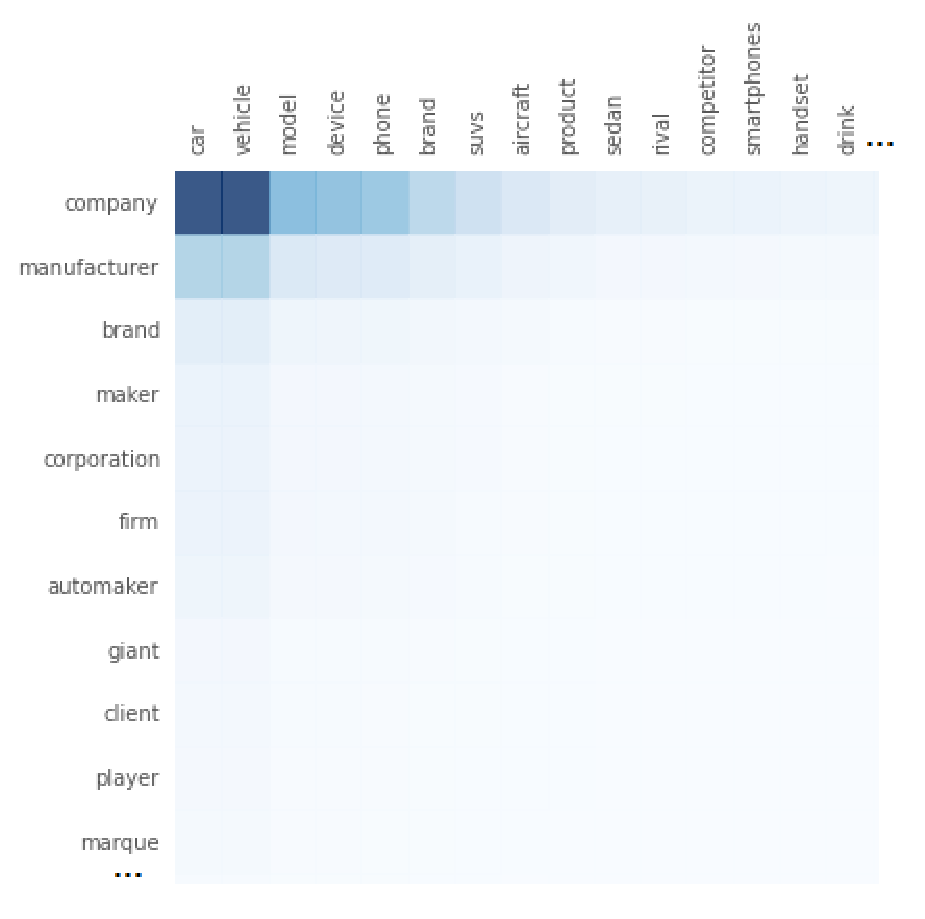
\epsfig{file=resources/ev_plot_manufacturer.eps,width=2.5in}
\caption{$\gamma_1,\gamma_2$) plot for attribute \term{Manufacturer}} \label{fig:evplot}
\end{figure}

\begin{example}[Sense Disambiguation]
Consider the following $(e1,a,e2)$ tuple \term{(iphone, manufacturer, apple)}. Suppose it is our query, where \term{apple}'s sense can either be a kind of \term{fruit} or a \term{company}.
Fig.~\ref{fig:evplot} is a heatmap for all the concepts pairs $(\gamma_1,\gamma_2)$ of attributes \term{manufacturer}. The horizontal axis represents the $e_1$ and the vertical axis stands for $e_2$. The darker the blue is, the higher typicality it will be. In Fig.~\ref{fig:evplot}, We can observe that the top concepts of $e_2$ in the heatmap are \term{company, manufacturer,...} and top 10 pairs also does not include \term{fruit}. The intuition for this is that there exists thousands of $(e1,a,e2)$ tuple such as \term{(BMW\_Z4,manufacturer,BMW),(PlayStation\_4,manufacturer,Sony)} other than \term{(iphone, manufacturer, apple)} tuple, which results in a reasonable distribution.
\label{exa:sd}
\end{example}


\subsection{Selectional Preference}

\subsection{Evaluation}